\section{Bisimulation equivalence}
% no \IEEEPARstart
Bisimulation equivalence (bisimilarity)\footnote{The notion of bisimulation equivalence (bisimilarity) in this chapter 
refers to strong bisimulation equivalence (strong bisimilarity)} is a binary relation between labeled transition systems 
which associates systems that can simulate each other's behaviour in a stepwise manner. This enables comparison of 
different transition systems.

An alternative perspective is to consider bisimulation equivalence as a relation between states of a single labelled 
transition system. By considering the quotient transition system under such a relation, smaller models are obtained
[BK08].

The bisimulation equivalence finds its extensive application in the area of formal verification of concurrent systems,
for example to check the equivalence of an implementation of a certain system with respect to its specification model.

In our tool the process of determining an existance of a bisimulation equivalence 
between two labeled transition systems was implemented using an approach which consists of three steps:

\begin{enumerate}
\item Computing strong bisimulation equivalence (strong bisimilarity) for each of the two LTSs;
\item Minimizing each of the two LTSs to its canonical form using the strong bisimilarity obtained
in the first step;
\item Performing a comparison between the two canonical forms obtained in the second step.
\end{enumerate}

The first step, computing strong bisimulation equivalence, was implemented with two different methods: the so called
naive method and a more efficient method due to Fernandez, both of which can serve as minimization procedures.

The naive algorithm [AILS07a] for computing bisimulation equivalence stems from the theory underlying Tarski's fixed point
theorem [AILS07b]. It has been proven that the strong bisimulation equivalence is the largest fixed point of the 
monotic function \mathcal{F} as defined in [AILS07a] given by Tarsky's fixed point theorem. 

This algorithm has time complexity of $O(mn)$ for a labeled transition system with
\emph{m} transitions and \emph{n} states. 

In our implementation the algorithm takes as input an LTS in aldebaran format, generates a corresponding labeled 
graph and then computes the strong bisimulation equivalence as pairs of bisimilar states.

The algorithm due to Fernandez exploits the idea of the relationship between strong bisimulation equivalence 
and the relational coarsest partition problem solved by Paige and Tarjan. It represents adaptation of the 
Paige-Tarjan algorithm of complexity $O(m \log n)$ to minimize labeled transition systems modulo bisimulation 
equivalence by computing the coarsest partition problem with respect to the family of binary relations 
$\left(T_a\right)_{a\in A}$ instead of one binary relation, where $T_a=\{(p,q)|(p,a,q)\in T\}$ is a transition 
relation for action ${a\in A}$ and $T$ is a set of all transitions [PT87, Fer89].

The algorithm due to Fernandez in our implementation takes an LTS in aldebaran format as an input, generates a 
corresponding labeled graph and then partitions the labeled graph into its coarsest blocks where each block represents 
a set of bisimilar states. Partition is a set of mutually exclusive blocks whose union constitutes the graph universe.

To define graph transitions the following terminology was used: 

\begin{itemize}
	\item $T_a[p]=\{q\}$ - an $a$-transition from state $p$ to state $q$
	\item $T_a{}^{-1}[q]=\{p\}$ - an inverse $a$-transition from state $q$ to state $p$
	\item $T_a{}^{-1}[B]=\cup \left\{T_a{}^{-1}[q],q\in B\right\}$ - inverse transition for block $B$ and action $a$
	\item $W$ - set of sets called splitters that are being used to split the partition
	\item infoB$(a, p)$ - info map for block $B$, state $p$ and action $a$
\end{itemize}

The time complexity of Fernandez's algorithm is $O(m \log n)$ for a labeled transition system 
with $m$ transitions and $n$ states. 

Both algorithms were implemented in Java. Several different data structures were used to implement the structure
labelled graph. The labelled graph is represented as a list of nodes. Each node is represented by the number of the
corresponding state, as a start state, and a list whose elements are couples of an outgoing action and a reachable 
state. 

% Sp = {(a, q)|a pripagja na A, q pripagja na Q, p ->a q}

% The algorithm of Fernandez requires additional data structures to represent the Ta, Ta_inversno (kako mnozestvo
% od trudot na Fernandez).

The next step uses the bisimulation equivalence computed in the first step in order to minimize the graphs. This reduction 
is implemented as follows:
\begin{enumerate}
	\item If a pair of states $(p, q)$ is bisimilar, then the two states are merged into one single state $k$;
	\item All incoming transitions $r \stackrel{a}{\rightarrow} p$ and $s \stackrel{a}{\rightarrow} q$ are replaced by transitions $r \stackrel{a}{\rightarrow} k$ and $s \stackrel{a}{\rightarrow} k$;
	\item All outgoing transitions $p \stackrel{a}{\rightarrow} r$ and $q \stackrel{a}{\rightarrow} s$ are replaced by transitions $k \stackrel{a}{\rightarrow} r$ and $k \stackrel{a}{\rightarrow} s$;
	\item The duplicate transitions are not taken into consideration.
\end{enumerate}
The procedure is repeated for all pairs of bisimilar states.

Having reduced the two labeled graphs into their minimal forms, the last step in the process of checking the equivalence
between the two labeled transition system consists of checking whether the two minimal labeled graphs are isomorphic.

Two graphs $G$ and $H$ are isomorphic if there exists a graph isomorphism between them. According to [BPS01], a graph isomorphism 
between two graphs G and H is a bijective function $f: Nodes(G) \rightarrow Nodes(H)$ satisfying:
\begin{itemize}
	\item $f(initialNode(G)) = g(initialNode(H))$
	\item $(s, a, t)$ is an edge in $G \Leftrightarrow (f(s), a, f(t))$ is an edge in $H$
\end{itemize}

The graph isomorphism check is implemented as follows:
Starting from the initial states, the outgoing tranzitions have to be the same, 
Povtorno pocnuvate od pocetnite sostojbi. Izleznite tranzicii mora da bidat isti, i za sekoja izlezna tranzicija so nekakva oznaka, mora da postoi druga takva so ista oznaka vo drugiot graf sto vodi povtorno do izomorfni sostojbi. Znaci treba da gi cuvate za sekoja sostojba nejzinite opcii za mozni izomorfni sostojbi. Posetenite sostojbi ne gi proveruvate (znaci ova e ednostavna rekurzija).

The two graphs are bisimilar.

The correctness of the implementation was tested with the use of ltsconvert and ltscompare tools of MCRL2, ....[ref6]

The whole process as described above is illustrated on the examples in Fig 

\begin{figure}[h!]
\centering
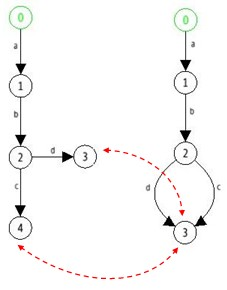
\includegraphics[width=2.0in]{bisimGraph2}
\caption{Minimized Graph 2}
\label{fig:bisimGraph2}
\end{figure}

\begin{figure}[h!]
\centering
\subfigure[Graph 1]{
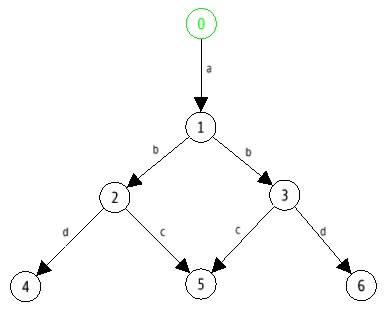
\includegraphics[width=2.3in]{graph1}
\label{fig:graph1}
}
\subfigure[Graph 2]{
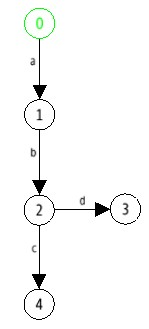
\includegraphics[width=0.9in]{graph2}
\label{fig:graph2}
}
\label{fig:exampleGraphs}
\caption{Example of two labeled graphs}
\end{figure}

\begin{figure}[h!]
\centering
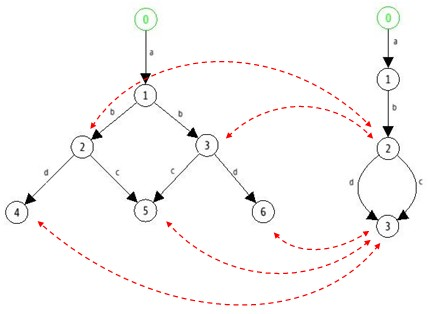
\includegraphics[width=3.0in]{bisimGraph1}
\caption{Minimized Graph 1}
\label{fig:bisimGraph1}
\end{figure}

An illustration of the output of the algorithms for the graphs shown on Fig. 2 and Fig. 3 is given in TABLE I.

\begin{table}[h!]
\begin{tabular}{| l | p{3.2cm}| p{3.2cm} | }
  \hline                       
  Algorithm & Graph 1 & Graph 2 \\ \hline
  Naive & \{(2, 3), (3, 2), (4, 5), 
(5, 4), (4, 6), (6, 4), (5, 6), (6, 5), (0, 0), (1, 1), (2, 2), (3, 3), (4, 4), (5, 5), (6, 6)\} & \{(3, 4), (4, 3), (0, 0), 
(1, 1), (2, 2), (3, 3), (4, 4)\} \\ \hline
  Fernandez & \{\{0\}, \{1\}, \{2\}, \{3\}, \{4, 5, 6\}\} & \{\{0\}, \{1\}, \{2\}, \{3, 4\}\} \\ \hline  
\end{tabular}
\caption{Computing strong bisimularity for Graph 1 and Graph 2}
\label{table1}
\end{table}

The process of reduction of the Graph 1 to its minimal form is given on Fig. 4. As it can be seen from the figure, the states 
2 and 3 are merged into state 2 in the minimal graph, and states 4, 5, and 6 are merged into state 3 in the minimal graph.
\begin{figure}[h!]
\centering
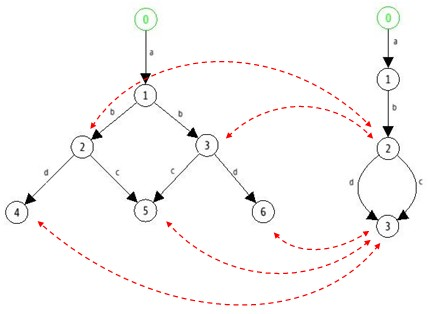
\includegraphics[width=3.0in]{bisimGraph1}
% where an .eps filename suffix will be assumed under latex, 
% and a .pdf suffix will be assumed for pdflatex; or what has been declared
% via \DeclareGraphicsExtensions.
\caption{Minimized Graph 1}
\label{fig:bisimGraph1}
\end{figure}

The process of reduction of the Graph 2 to its minimal form is given on Fig. 5. As before, the states 
3 and 4 are merged into state 3 in the minimal graph.
\begin{figure}[h!]
\centering
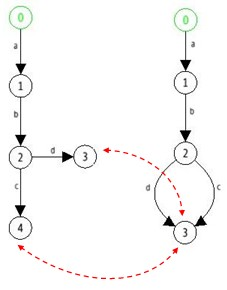
\includegraphics[width=1.8in]{bisimGraph2}
% where an .eps filename suffix will be assumed under latex, 
% and a .pdf suffix will be assumed for pdflatex; or what has been declared
% via \DeclareGraphicsExtensions.
\caption{Minimized Graph 2}
\label{fig:bisimGraph2}
\end{figure}

% [ref6}: url za mcrl2
% [ref7]: Model checking